%==============================================================
%  Figura 6.14 - Riordino dei sottosistemi misti nello schema a
%  blocchi legato alla sicurezza
%  Adattamento in italiano della Figura 6.14 dell'IFA Report 2/2017
%
%  Coordinate ricavate dalla grafica vettoriale dell'originale
%  (pagina 74 di rep0217e.pdf), espresse nei punti PostScript di quel
%  disegno; con x=y=0.035cm una unita' vale circa un punto TeX, quindi
%  i corpi dei caratteri sono gli stessi dell'originale.
%
%  Sistema di riferimento: l'origine e' l'angolo in basso a sinistra
%  della cornice; l'asse y e' rivolto verso l'alto.
%
%  Lo schema in alto e' quello "fisico" (tre sottosistemi: la coppia
%  I1/I2, il blocco L incapsulato, la coppia O1/O2); quello in basso e'
%  lo stesso sistema riordinato dando la precedenza a L, che lo riduce
%  a due sottosistemi. La freccia grigia indica il riordino.
%==============================================================
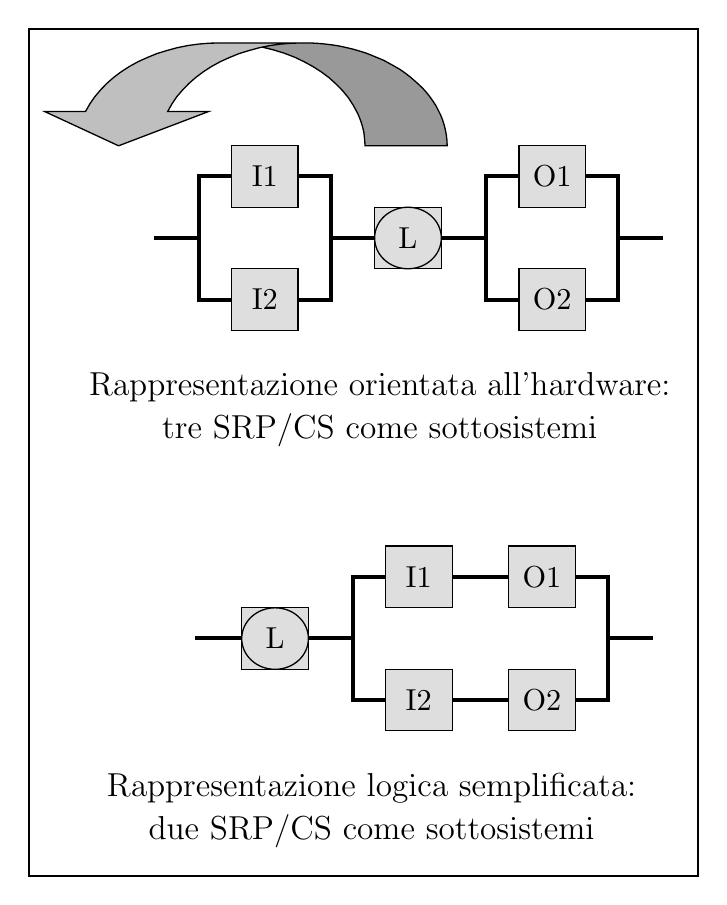
\begin{tikzpicture}[
  x=0.035cm, y=0.035cm,
  cornice/.style={draw=black, line width=0.75pt},
  blocco/.style={draw=black, fill=black!13, line width=0.47pt},
  collegamento/.style={draw=black, line width=1.49pt},
  sigla/.style={font=\fontsize{11.3}{13.5}\selectfont},
  dicitura/.style={font=\fontsize{13}{15.5}\selectfont, align=center}
]

\setstretch{1}

% --- freccia curva del riordino (conversione dai tracciati originali) ---
\fill[fill=black!25] (32.98,265.37) -- (65.7,277.83) -- (50.79,277.83) -- (52.37,280.6) -- (54.11,283.2) -- (56.23,285.64) -- (58.52,288.01) -- (61.05,290.22) -- (63.8,292.26) -- (66.72,294.16) -- (69.88,295.89) -- (73.19,297.39) -- (76.66,298.81) -- (80.28,299.92) -- (84,300.94) -- (87.86,301.73) -- (91.88,302.28) -- (95.9,302.6) -- (100,302.67) -- (70.19,302.67) -- (66.09,302.6) -- (62.07,302.28) -- (58.05,301.73) -- (54.18,300.94) -- (50.48,299.92) -- (46.85,298.81) -- (43.39,297.39) -- (40.07,295.89) -- (36.92,294.16) -- (34,292.26) -- (31.24,290.22) -- (28.72,288.01) -- (26.43,285.64) -- (24.38,283.2) -- (22.57,280.6) -- (20.99,277.83) -- (6.09,277.83) -- cycle;
\fill[fill=black!40] (85.1,301.18) -- (89.2,300.15) -- (93.06,298.97) -- (96.77,297.55) -- (100.24,295.89) -- (103.55,294.08) -- (106.62,292.11) -- (109.46,289.98) -- (111.99,287.69) -- (114.36,285.25) -- (116.4,282.73) -- (118.14,280.04) -- (119.63,277.28) -- (120.26,275.86) -- (120.81,274.44) -- (121.29,272.94) -- (121.68,271.53) -- (122,270.03) -- (122.16,268.45) -- (122.31,266.95) -- (122.39,265.37) -- (152.2,265.37) -- (152.12,267.35) -- (151.89,269.24) -- (151.57,271.05) -- (151.1,272.94) -- (150.54,274.76) -- (149.84,276.5) -- (148.96,278.23) -- (148.1,279.96) -- (147,281.62) -- (145.89,283.2) -- (144.63,284.78) -- (143.29,286.27) -- (141.79,287.69) -- (140.21,289.11) -- (138.64,290.45) -- (136.9,291.79) -- (135.09,293.06) -- (133.19,294.16) -- (129.17,296.37) -- (124.84,298.18) -- (122.63,299.05) -- (120.34,299.76) -- (117.9,300.47) -- (115.54,301.02) -- (113.01,301.57) -- (110.49,301.97) -- (107.96,302.28) -- (105.36,302.52) -- (102.68,302.67) -- (100,302.67) -- (96.21,302.6) -- (92.51,302.28) -- (88.73,301.81) -- cycle;
\draw[draw=black, line width=0.47pt] (85.1,301.18) -- (89.2,300.15) -- (93.06,298.97) -- (96.76,297.55) -- (100.24,295.89) -- (103.55,294.08) -- (106.62,292.11) -- (109.46,289.98) -- (111.98,287.69) -- (114.35,285.25) -- (116.4,282.73) -- (118.13,280.04) -- (119.63,277.28) -- (120.26,275.86) -- (120.82,274.44) -- (121.29,272.94) -- (121.68,271.53) -- (122,270.03) -- (122.16,268.45) -- (122.31,266.95) -- (122.39,265.37) -- (152.2,265.37) -- (152.12,267.35) -- (151.89,269.24) -- (151.57,271.05) -- (151.1,272.94) -- (150.54,274.76) -- (149.84,276.5) -- (148.1,279.96) -- (147,281.62) -- (145.89,283.2) -- (144.63,284.78) -- (143.29,286.27) -- (141.79,287.69) -- (140.21,289.11) -- (138.64,290.45) -- (136.9,291.79) -- (135.09,293.06) -- (133.19,294.16) -- (129.18,296.37) -- (124.84,298.18) -- (122.63,299.05) -- (120.34,299.76) -- (117.9,300.47) -- (115.53,301.02) -- (113.01,301.57) -- (110.48,301.97) -- (107.96,302.28) -- (105.36,302.52) -- (102.68,302.67) -- (70.19,302.67) -- (66.09,302.6) -- (62.07,302.28) -- (58.05,301.73) -- (54.18,300.94) -- (50.48,299.92) -- (46.85,298.81) -- (43.39,297.39) -- (40.07,295.89) -- (36.92,294.16) -- (34,292.27) -- (31.24,290.22) -- (28.72,288.01) -- (26.43,285.64) -- (24.38,283.2) -- (22.57,280.6) -- (20.99,277.83) -- (6.09,277.83) -- (32.98,265.37) -- (65.7,277.83) -- (50.79,277.83) -- (52.37,280.6) -- (54.11,283.2) -- (56.23,285.64) -- (58.52,288.01) -- (61.05,290.22) -- (63.8,292.27) -- (66.72,294.16) -- (69.88,295.89) -- (73.19,297.39) -- (76.66,298.81) -- (80.29,299.92) -- (84,300.94) -- (87.86,301.73) -- (91.88,302.28) -- (95.9,302.6) -- (100,302.67);

% ===================== schema in alto: tre sottosistemi =====================
% linee portanti
\draw[collegamento] (45.91,231.87) -- (62.78,231.87);
\draw[collegamento] (150.15,231.87) -- (167.02,231.87);
\draw[collegamento] (213.62,231.87) -- (230.50,231.87);
% staffe dei due canali
\draw[collegamento] (74.06,254.26) -- (62.15,254.26) -- (62.15,209.55) -- (74.06,209.55);
\draw[collegamento] (98.10,254.26) -- (109.94,254.26) -- (109.94,209.55) -- (98.10,209.55);
\draw[collegamento] (178.30,254.26) -- (166.39,254.26) -- (166.39,209.55) -- (178.30,209.55);
\draw[collegamento] (202.35,254.26) -- (214.18,254.26) -- (214.18,209.55) -- (202.35,209.55);
% tratto fra la staffa di ingresso e il blocco L
\draw[collegamento] (109.38,231.87) -- (125.86,231.87);
% blocchi
\draw[blocco] (73.98,243.07) rectangle (98.10,265.38);
\draw[blocco] (178.22,243.07) rectangle (202.35,265.38);
\draw[blocco] (73.98,198.35) rectangle (98.10,220.75);
\draw[blocco] (178.22,198.35) rectangle (202.35,220.75);
% sottosistema incapsulato: cerchio inscritto nel quadrato
\draw[blocco] (125.86,220.75) rectangle (150.07,243.07);
\draw[blocco] (137.97,231.91) ellipse [x radius=12.1, y radius=11.16];
% sigle
\node[sigla] at (86.04,254.22) {I1};
\node[sigla] at (190.29,254.22) {O1};
\node[sigla] at (137.97,231.91) {L};
\node[sigla] at (86.04,209.55) {I2};
\node[sigla] at (190.29,209.55) {O2};
% dicitura
\node[dicitura] at (127.73,169.62)
  {Rappresentazione orientata all'hardware:\\tre SRP/CS come sottosistemi};

% ================= schema in basso: due sottosistemi =================
\draw[collegamento] (60.81,86.63) -- (77.68,86.63);
\draw[collegamento] (101.81,86.63) -- (118.69,86.63);
\draw[collegamento] (209.92,86.63) -- (226.79,86.63);
\draw[collegamento] (154.01,108.93) -- (174.59,108.93);
\draw[collegamento] (154.01,64.23) -- (174.59,64.23);
\draw[collegamento] (129.81,108.94) -- (117.90,108.94) -- (117.90,64.23) -- (129.81,64.23);
\draw[collegamento] (198.64,108.94) -- (210.47,108.94) -- (210.47,64.23) -- (198.64,64.23);
% blocchi
\draw[blocco] (129.73,97.74) rectangle (154.01,120.13);
\draw[blocco] (174.51,97.74) rectangle (198.64,120.13);
\draw[blocco] (129.73,53.11) rectangle (154.01,75.42);
\draw[blocco] (174.51,53.11) rectangle (198.64,75.42);
\draw[blocco] (77.60,75.42) rectangle (101.89,97.74);
\draw[blocco] (89.75,86.58) ellipse [x radius=12.1, y radius=11.16];
% sigle
\node[sigla] at (141.87,108.93) {I1};
\node[sigla] at (186.58,108.93) {O1};
\node[sigla] at (89.75,86.58) {L};
\node[sigla] at (141.87,64.26) {I2};
\node[sigla] at (186.58,64.26) {O2};
% dicitura
\node[dicitura] at (124.73,24.12)
  {Rappresentazione logica semplificata:\\due SRP/CS come sottosistemi};

% --- cornice esterna --------------------------------------------------------
\draw[cornice] (0.37,0.37) rectangle (243.11,307.85);

\end{tikzpicture}
